\documentclass{scrreprt}
\usepackage{array}
\usepackage{graphicx}
\usepackage{listings}
\usepackage{underscore}
\usepackage[bookmarks=true]{hyperref}
\usepackage[utf8]{inputenc}
\usepackage{float}
\usepackage[french]{babel}
\hypersetup{
    bookmarks=false,    % show bookmarks bar
    pdftitle={rapport_TP1_Lambolez_Petit},    % title
    pdfauthor={Théodore Lambolez, Maximilien Petit},                     % author
    pdfsubject={TeX and LaTeX},                        % subject of the document
    pdfkeywords={TeX, LaTeX, graphics, images}, % list of keywords
    colorlinks=true,       % false: boxed links; true: colored links
    linkcolor=blue,       % color of internal links
    citecolor=black,       % color of links to bibliography
    filecolor=black,        % color of file links
    urlcolor=black,        % color of external links
    linktoc=page            % only page is linked
}
\def\myversion{1.0}
\date{}
%\title
\usepackage{hyperref}
\begin{document}
\begin{figure}
   \begin{minipage}[c]{.46\linewidth}
      
\includegraphics[scale=0.3]{images/telecom.png}
   \end{minipage} \hfill
   \begin{minipage}[c]{.46\linewidth}
      
\includegraphics[scale=1.9]{images/lorraine.jpg}
   \end{minipage}
\end{figure}
\begin{flushright}
    \rule{15cm}{5pt}
    \vskip1cm
\end{flushright}
\begin{center}
	\vspace{3cm}
	\fbox{
	\begin{minipage}{0.9\textwidth}
        	\Huge{
			\textbf{
			\begin{center}
				Rapport \\Travaux Pratiques 3
				\vspace{0.5cm}
			\end{center}
			}
		}
	\end{minipage}
	}
\end{center}
\begin{flushright}
        \vspace{5cm}
	\huge{
        \textbf{
	Ecrit par \\
	\vspace{0,875cm}
	\href{mailto:theodore.lambolez@telecomnancy.eu}{Théodore Lambolez} \\
	\href{mailto:maximilien.petit@telecomnancy.eu}{Maximilien Petit}\\
	}
	}
        \vspace{0,5cm}
        \large{
	\textbf{
	\today\\
	}	
	}
\end{flushright}

\tableofcontents

\chapter{Classification appliquée à la reconnaissance d'objets}

\paragraph{Introduction :}
Le but de ce troisième et dernier TP de Traitement Numérique de l'Image est
de réaliser une macro sur le logiciel Optimas qui permettra de reconnaitre 
des objets présents sur la scène capturée. 
Comme toujours, il faut préciser les hypothèses de 
bases. Ici, nous faisons en sorte que le capteur prenne toujours la 
scène avec le même angle d'inclinaison et avec la même distance de celle-ci.
La macro est présente dans la partie "Annexe".

\paragraph{Manipulations préalables :}
Avant d'utiliser cette macro, il est impératif de s'assurer que la
calibration nommée "One_pixel_per_centimeter" 

\paragraph{Méthode mise en oeuvre :}
Ici, avant toute chose, nous nous assurons que l'option de calibration nommée
"One_pixel_per_centimeter" soit bien selectionnée. 

Ensuite, comme pour les précédentes macros réalisées sur Optimas, nous commencerons
par réaliser une binarisation de l'image. Il faut donc définir un seuil, 
qui devra s'adapter à l'image. C'est pourquoi, on a choisi d'utiliser une
nouvelle fois l'outil nommé "auto-threshold". Ici, en raison du nombre d'objets
présent sur les images, nous avons choisi d'utiliser l'option de détection du seuil
par modélisation d'une exponentielle décroissante. 

Une fois l'image binarisée, on constate que certains objets sont séparés en plusieurs
ou bien que d'autres présentent des évidements. Afin de faciliter la classification, 
il est important de mettre en oeuvre une solution pour les rassembler et les reboucher.
Nous avons choisi d'utiliser des opérations de morphologie mathématiques pour ce faire.
En effet, nous réalisons successivement une fermeture et une ouverture. 

Il est maintenant temps de passer à la séparation des objets et à leur identifications.
Pour ce faire, on débute en paramétrant le "Data Sampling Area" de telle sorte que la 
détection de contour se fera en 8-voisinage en prenant en compte les évidements. On spécifiera 
également une longueur minimale de frontière intérieure de 5 pixels et le fait qu'on ne 
prend pas en compte les objets présents au niveau des bords de l'image. En effet, 
si les objets touchent le bord, on ne peut pas être certain que celui-ci est complet. 
Cela faussera potentiellement son identification. 

Ensuite, on utilise l'outil "Particules Count" dans le but de mettre en évidence les différentes
régions isolées avec le paramétrage précédant. Ces régions isolées correspondent aux différents
objets. 

Afin de les identifier, il faut créer une nouvelle classe pour chacun des types d'objets
que l'on souhaite identifier et une dernière classe correspondant aux objets que l'on ne
souhaite pas identifier. 

Enfin, nous nous assurerons de l'extraction de toutes les données nécessaires à la classification
à l'aide du "Measurment Explorer".

\paragraph{Critère choisis pour les 9 classes créées :}

\begin{table}[!h]
        \begin{center}
                \begin{tabular}{|c|c|c|c|c|c|c|}
                   \hline
                   Nom classe & Nb Euler & Nb Parents & Circularité & Rectangularité & Région &  Largeur \\
                   \hline
		   Clés & 1 & & > 80 & & > 3500 & < 100 \\
		   \hline
		   Rondelles & 0 & 0 & < 30 & < 0.65 & & \\
		   \hline
		   Dés face 1 & 0 & 0 & < 30 & < 0.65 & & \\
		   \hline
                   Dés face 2 & -1 & 0 & < 30 & < 0.65 & & \\
                   \hline
                   Dés face 3 & -2 & 0 & < 30 & < 0.65 & & \\
                   \hline
                   Dés face 4 & -3 & 0 & < 30 & < 0.65 & & \\
                   \hline
                   Dés face 5 & -4 & 0 & < 30 & < 0.65 & & \\
                   \hline
                   Dés face 6 & -5 & 0 & < 30 & < 0.65 & & \\
                   \hline
		   Objets & 1 & 0 &  18 < x < 22 & > 0.65 & & \\
		   robotiques & & & & & &\\
                   \hline 
                \end{tabular}
        \end{center}
        \caption{Tableau des critères choisis (hors classe Intrus)}
\end{table}
  
Pour ce qui est de la dernière classe correspondant aux objets que nous ne souhaitons
pas identifier, nous avons simplement pris tous les objets n'appartenant à aucune des classes
précédentes.

\newpage
\paragraph{Analyse des résultats :}
 
Nous allons dans ce paragraphe analyser les résultats de notre macro pour différentes images.

\begin{figure}[!h]
\centering
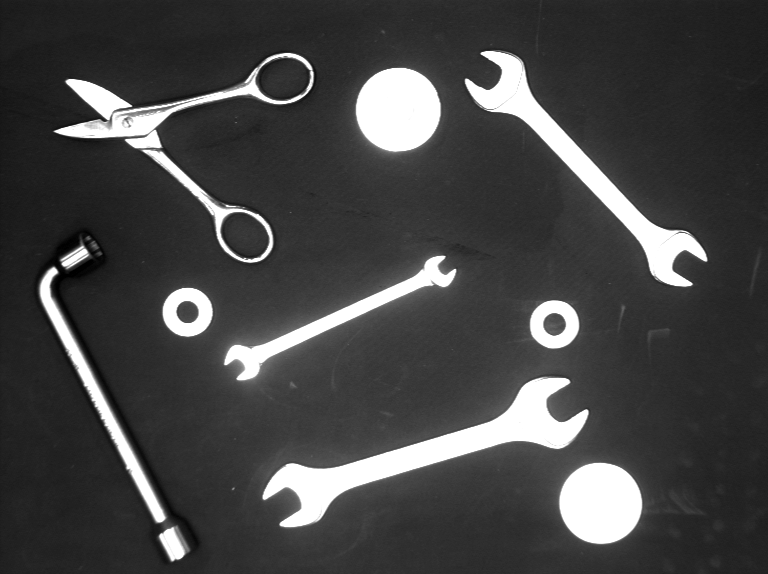
\includegraphics[width=5cm, height=5cm]{images/objet1o.png}\hfill
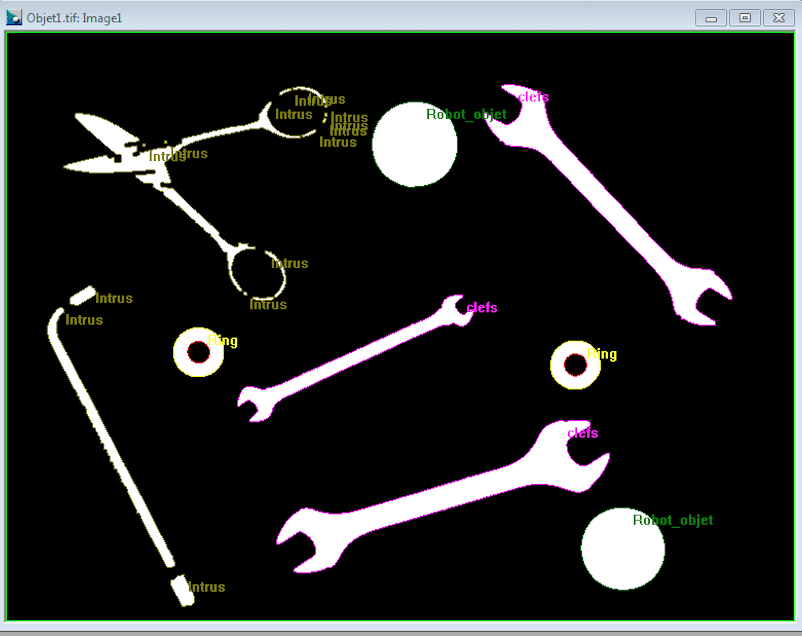
\includegraphics[width=5cm, height=5cm]{images/objet1.png}
\caption{Résultat de l'identification d'objets avec la macro sur l'image Objets1.tif}
\end{figure}

On peut constater sur cette image que tous les objets que l'on veut identifier ont bien 
été identifiés. Néanmoins, si on voulait identifier les ciseaux, l'étape de reformation 
des objets ici proposée n'est pas suffisante afin de rassembler toutes les parties de cet
objet détachées par la binarisation. On pourrait également tenter d'améliorer le seuil 
de binarisation choisi.  

\begin{figure}[!h]
\centering
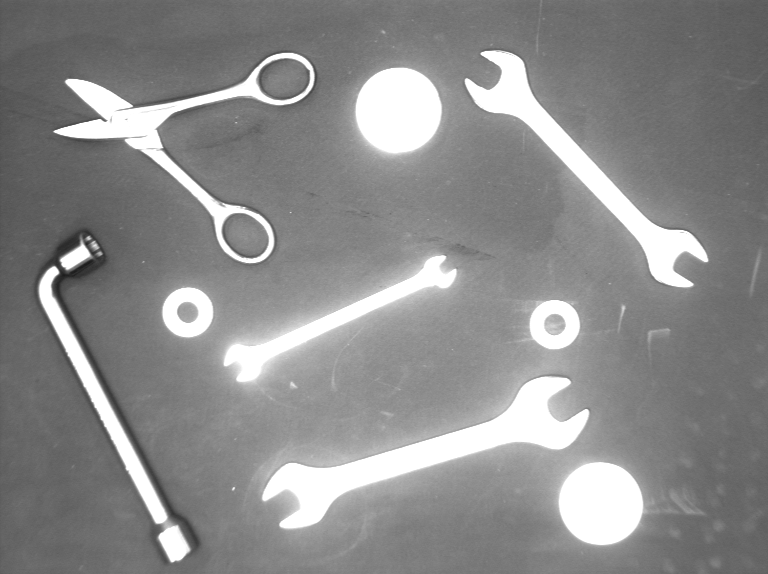
\includegraphics[width=5cm, height=5cm]{images/objet1Lo.png}\hfill
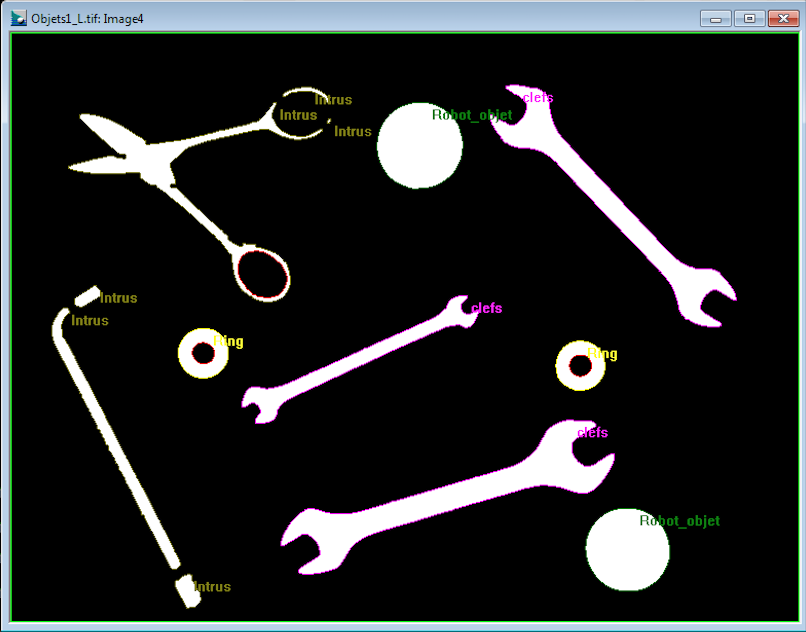
\includegraphics[width=5cm, height=5cm]{images/objet1L.png}
\caption{Résultat de l'identification d'objets avec la macro sur l'image Objets1_L.tif}
\end{figure}

Sur cette image dont la scène est davantage éclairée, on peut constater qu'une bonne partie
des ciseaux a été reformée. On constate également que le fort éclairage n'a pas influencé 
le résultat de notre identification des objets souhaités. 

\newpage
De même, un faible éclairement de cette scène n'affecte pas notre résultat.

\begin{figure}[!h]
\centering
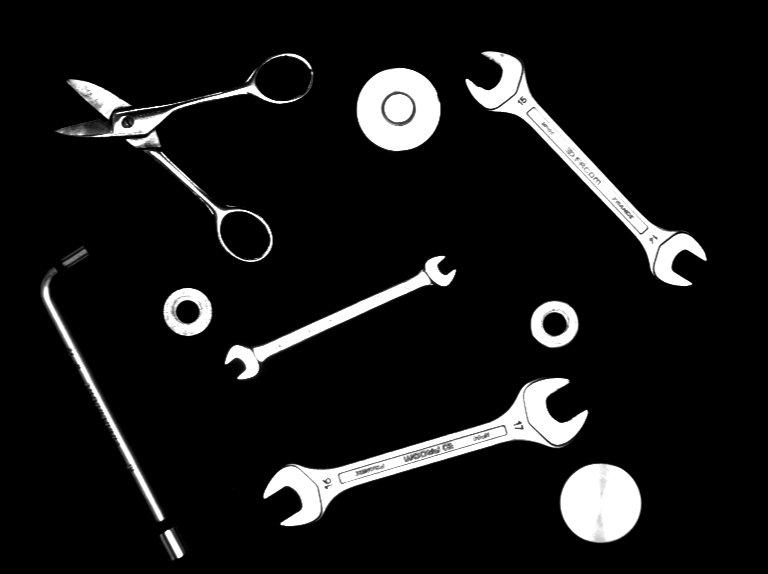
\includegraphics[width=5cm, height=5cm]{images/objet1Do.png}\hfill
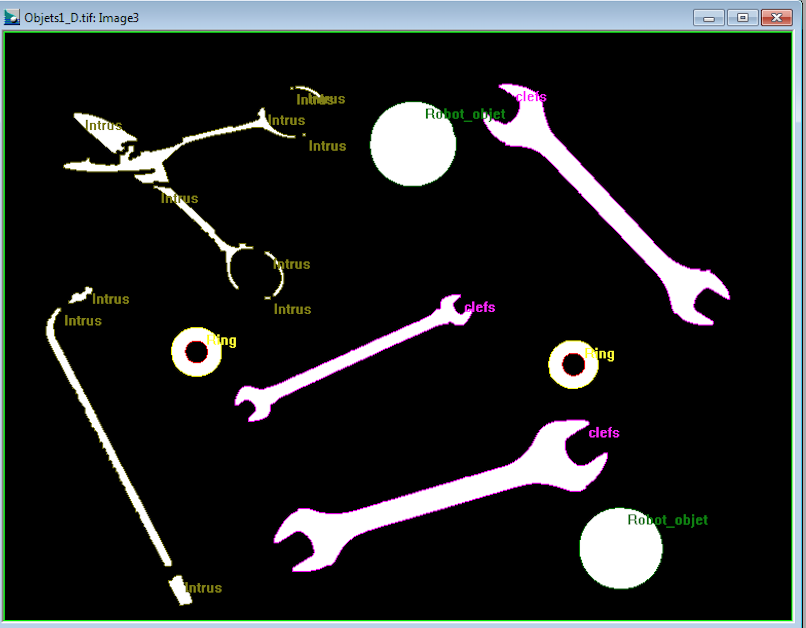
\includegraphics[width=5cm, height=5cm]{images/objet1D.png}
\caption{Résultat de l'identification d'objets avec la macro sur l'image Objets1_D.tif}
\end{figure}


\begin{figure}[!h]
\centering
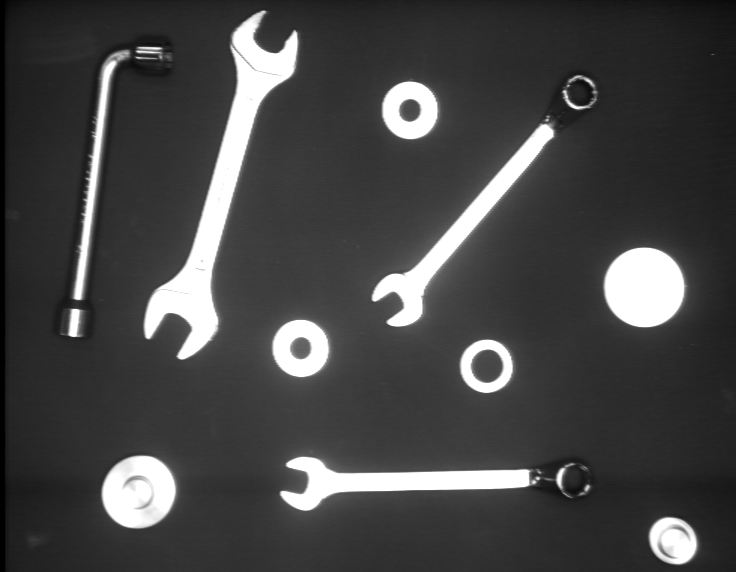
\includegraphics[width=5cm, height=5cm]{images/objet2o.png}\hfill
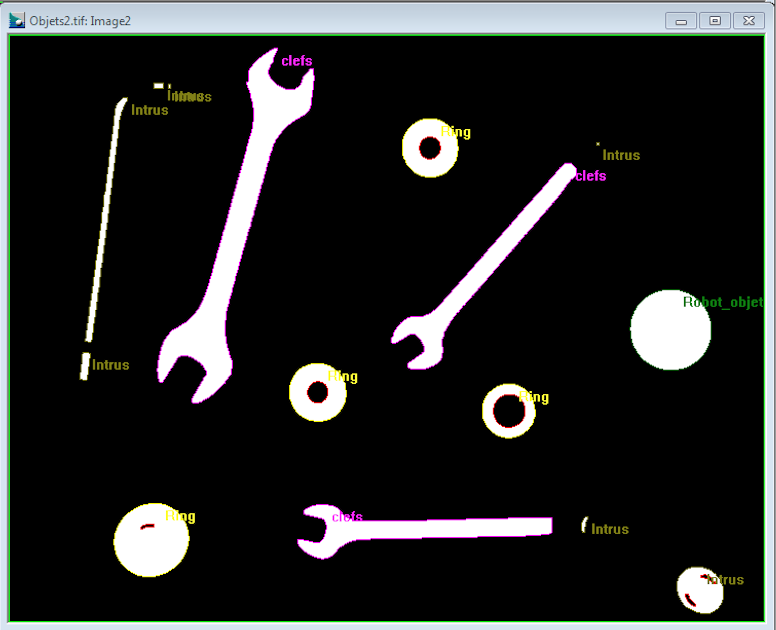
\includegraphics[width=5cm, height=5cm]{images/objet2.png}
\caption{Résultat de l'identification d'objets avec la macro sur l'image Objets2.tif}
\end{figure}

Le résultat de la macro pour cette image apporte une nouvelle limite. En effet, on
constate qu'une pièce robotique est identifiée comme une rondelle. Ce problème est du
à un phénomène d'ombre portée. En fait, le fait que le capteur ne soit pas exactement 
au dessus de cette pièce, fait que le bord est suffisamment important pour être capté.
Comme une ombre est plus foncée que l'objet en lui-même, la binarisation globale de l'image
revient à considérer ces pixels comme du fond. D'où le nombre d'Euler égal à 0 (1 -1 évidement)
impliquant selon la classification réalisée, qu'on a affaire à une rondelle et non à 
une pièce robotique.  


\newpage
Ici, le fort éclairage de la scène, augmente le constrate entre les pièces et cette portée.
Par conséquent, le phénomène mis en évidence précédemment est amplifié. 

\begin{figure}[!h]
\centering
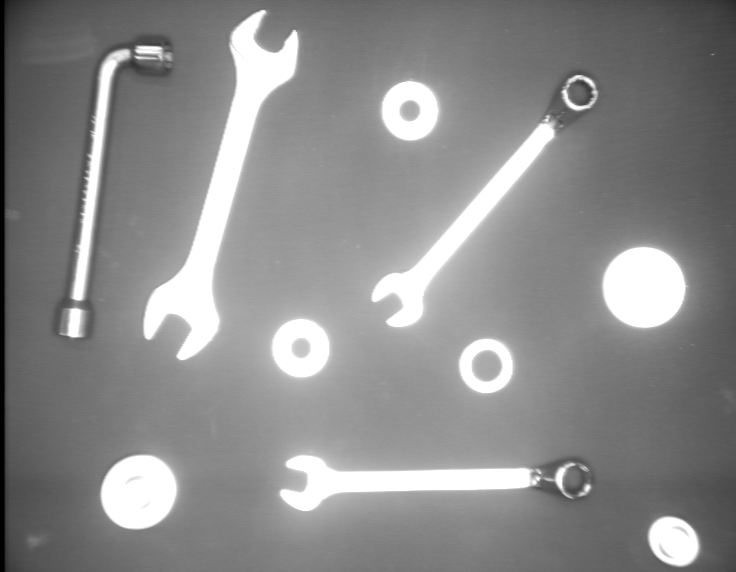
\includegraphics[width=5cm, height=5cm]{images/objet2Lo.png}\hfill
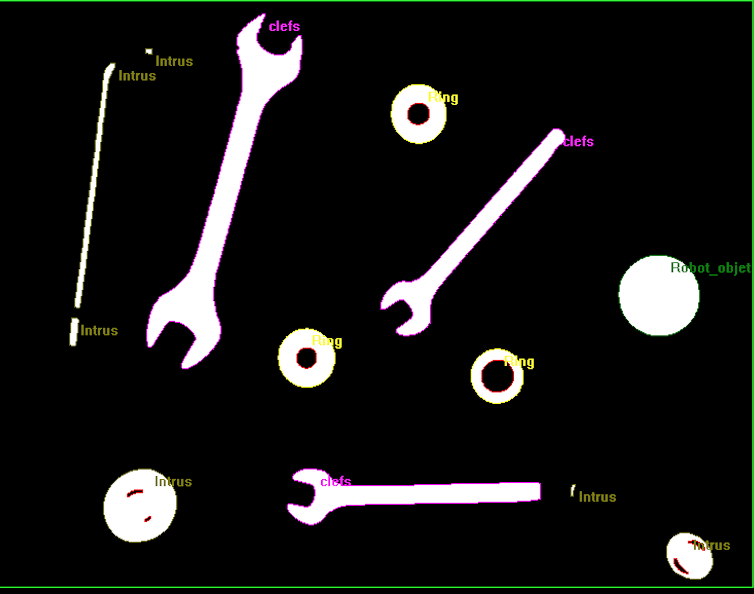
\includegraphics[width=5cm, height=5cm]{images/objet2L.png}
\caption{Résultat de l'identification d'objets avec la macro sur l'image Objets2_L.tif}
\end{figure}


\begin{figure}[!h]
\centering
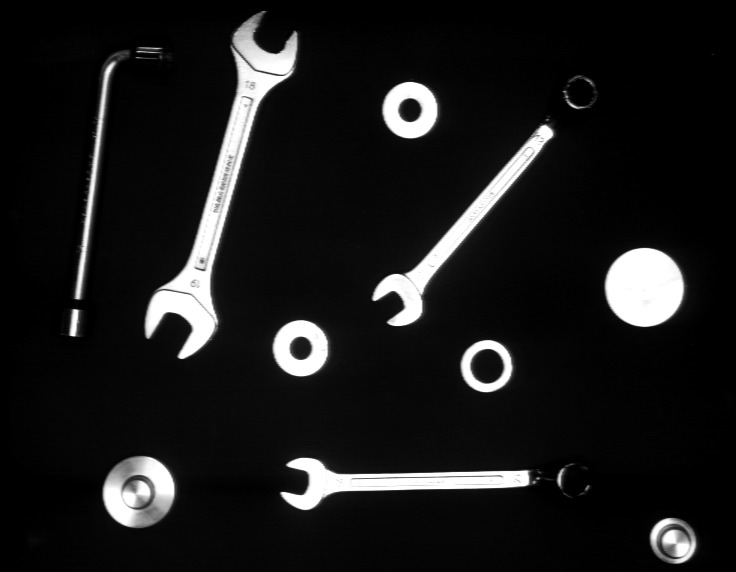
\includegraphics[width=5cm, height=5cm]{images/objet2Do.png}\hfill
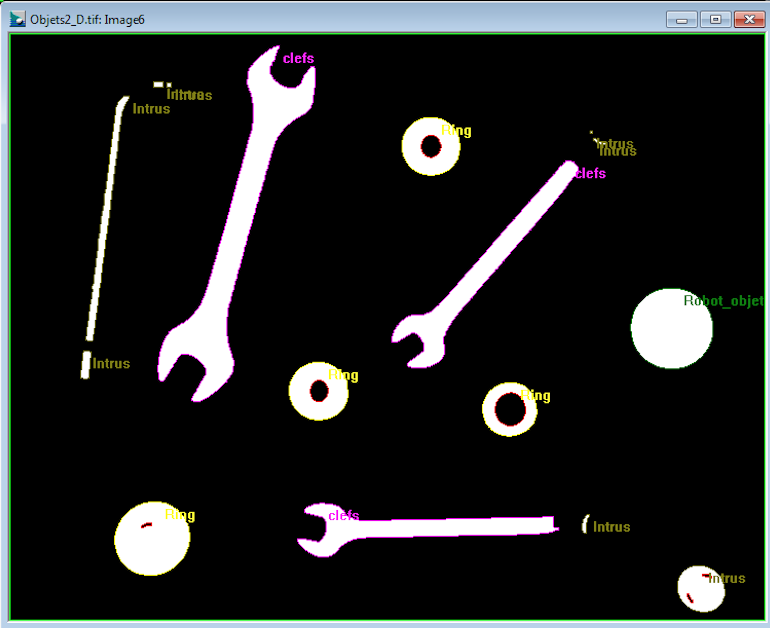
\includegraphics[width=5cm, height=5cm]{images/objet2D.png}
\caption{Résultat de l'identification d'objets avec la macro sur l'image Objets2_D.tif}
\end{figure}

Dans ce cas où la scène est plus sombre, on constate une légère amélioration.
Cependant, elle n'est pas suffisante.

\newpage
Pour cette image, la macro réalise le travail espéré.
\begin{figure}[!h]
\centering
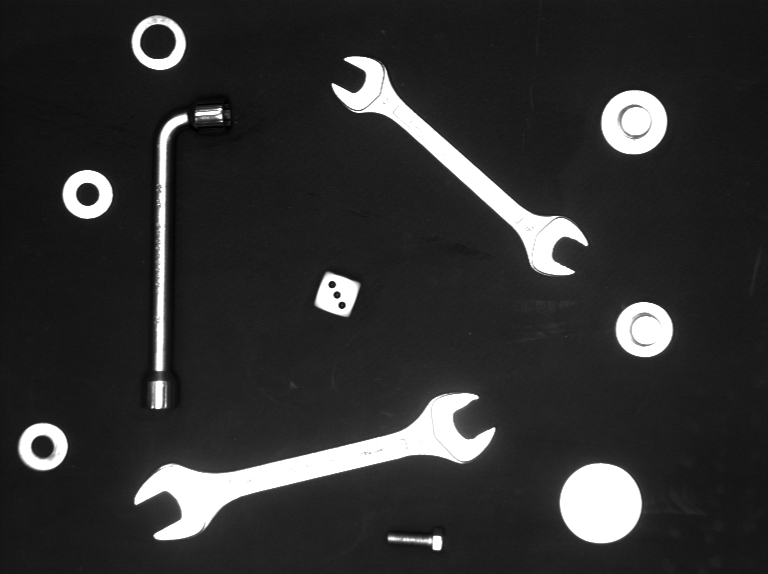
\includegraphics[width=5cm, height=5cm]{images/objet3o.png}\hfill
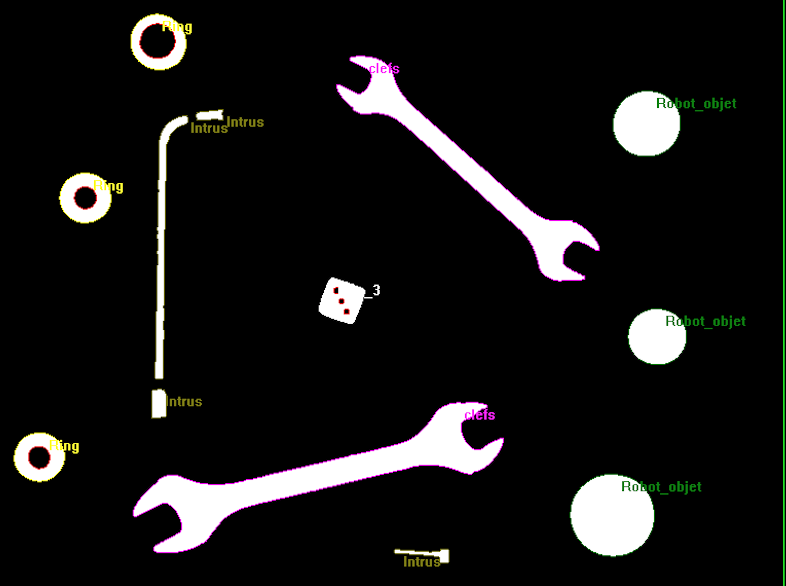
\includegraphics[width=5cm, height=5cm]{images/objet3.png}
\caption{Résultat de l'identification d'objets avec la macro sur l'image Objets3.tif}
\end{figure}

Le résultat sur l'image Objets4.tif, révèle un autre problème dans notre classification.
En effet, nous n'avons pas réussi à ne pas identifier la moitié de clé comme n'en étant 
pas une. Il faudrait réaliser une classification dont les bornes seraient plus rapprochées 
afin de ne plus l'identifier. Néanmoins, en changeant les valeurs choisie, la classification
pour les autres images risque de ne plus être bonne. 
\begin{figure}[!h]
\centering
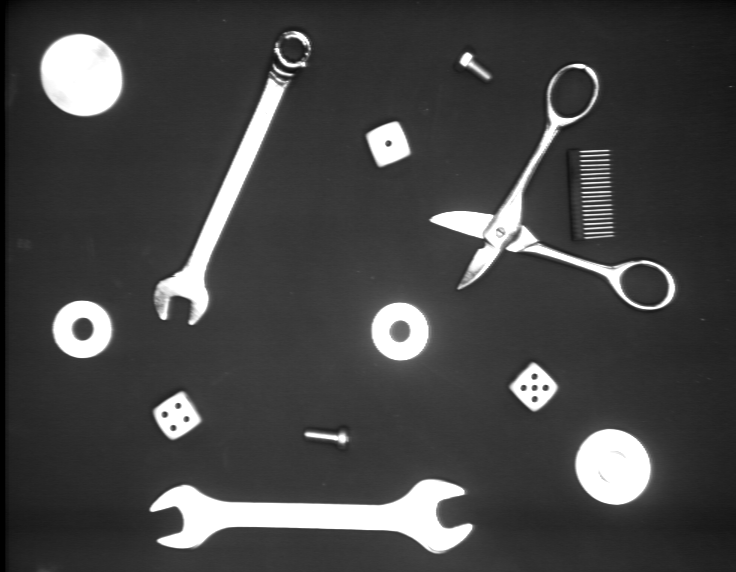
\includegraphics[width=5cm, height=5cm]{images/objet4o.png}\hfill
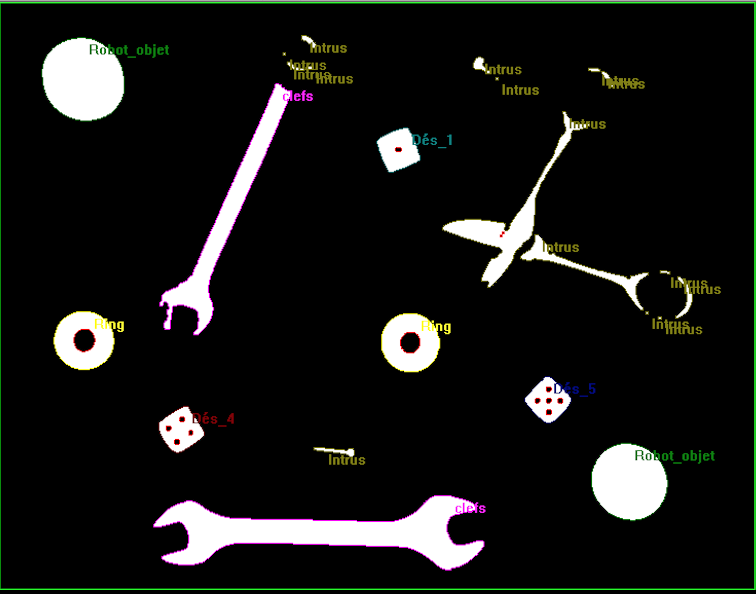
\includegraphics[width=5cm, height=5cm]{images/objet4.png}
\caption{Résultat de l'identification d'objets avec la macro sur l'image Objets4.tif}
\end{figure}

\newpage
Nous avons le même problème pour le stylet métalique présent sur cette image. 
Notre classification mène à considérer cet objet comme une clé. 
\begin{figure}[!h]
\centering
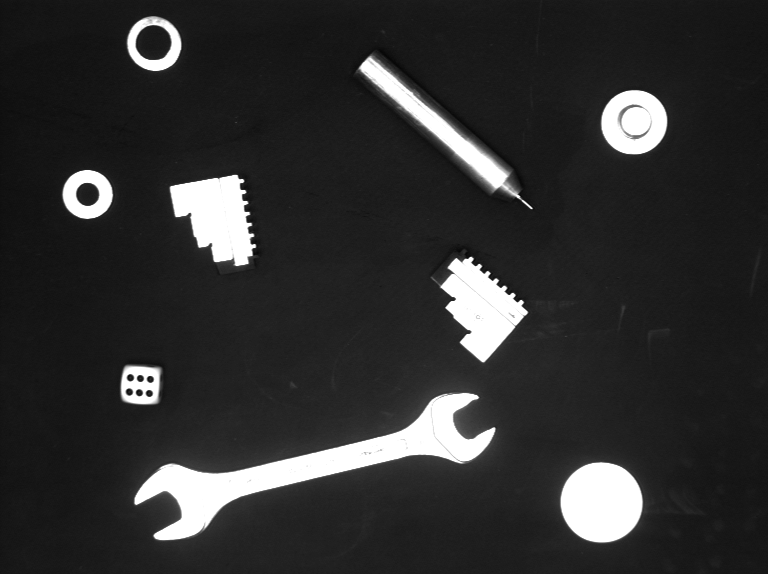
\includegraphics[width=5cm, height=5cm]{images/objet5o.png}\hfill
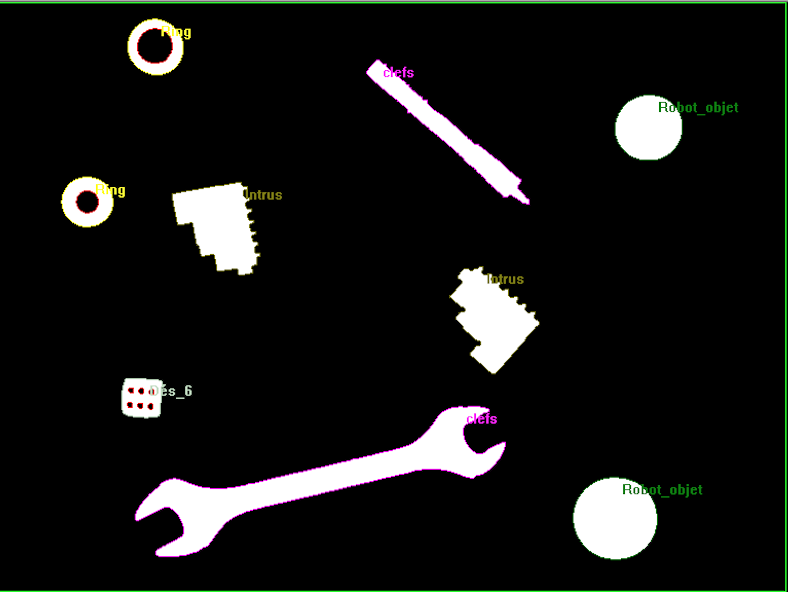
\includegraphics[width=5cm, height=5cm]{images/objet5.png}
\caption{Résultat de l'identification d'objets avec la macro sur l'image Objets5.tif}
\end{figure}

Les derniers résultats présentés n'apportent aucune nouvelle limite à notre macro.
\begin{figure}[!h]
\centering
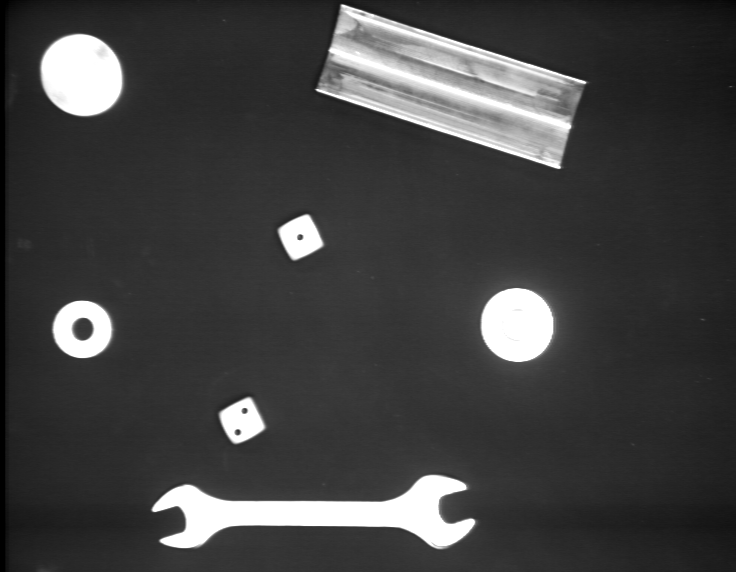
\includegraphics[width=5cm, height=5cm]{images/objet6o.png}\hfill
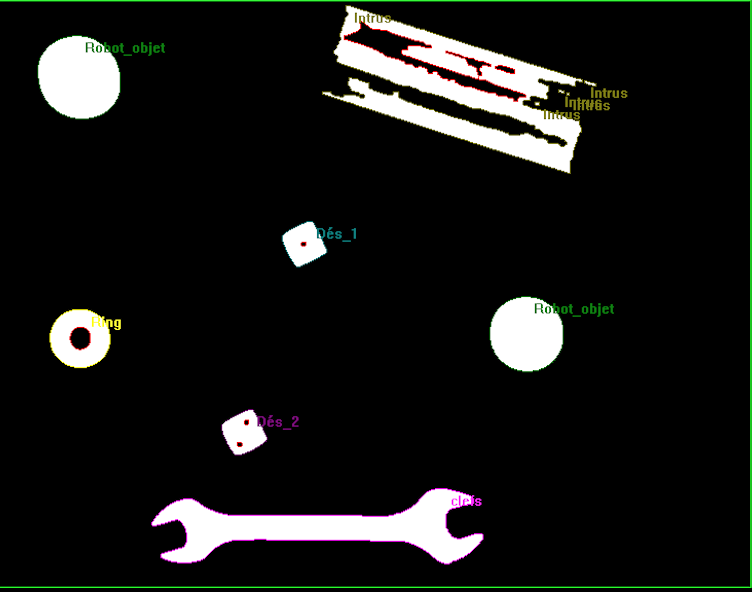
\includegraphics[width=5cm, height=5cm]{images/objet6.png}
\caption{Résultat de l'identification d'objets avec la macro sur l'image Objets6.tif}
\end{figure}

\begin{figure}[!h]
\centering
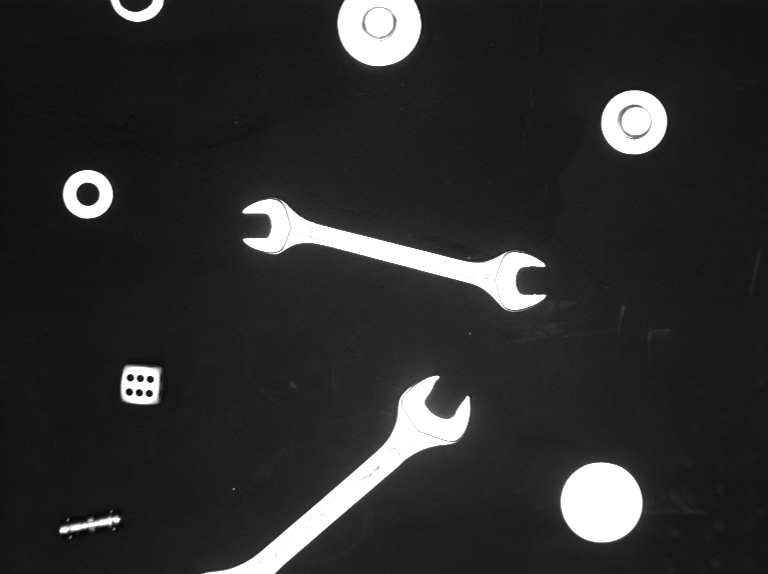
\includegraphics[width=5cm, height=5cm]{images/objet7o.png}\hfill
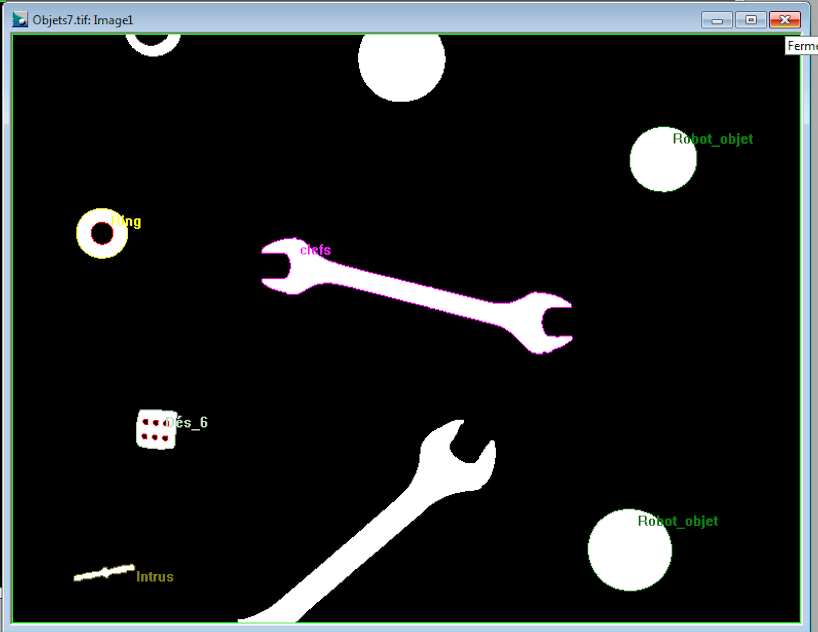
\includegraphics[width=5cm, height=5cm]{images/objet7.png}
\caption{Résultat de l'identification d'objets avec la macro sur l'image Objets7.tif}
\end{figure}

\chapter{Annexe}

\begin{figure}[!h]
\centering
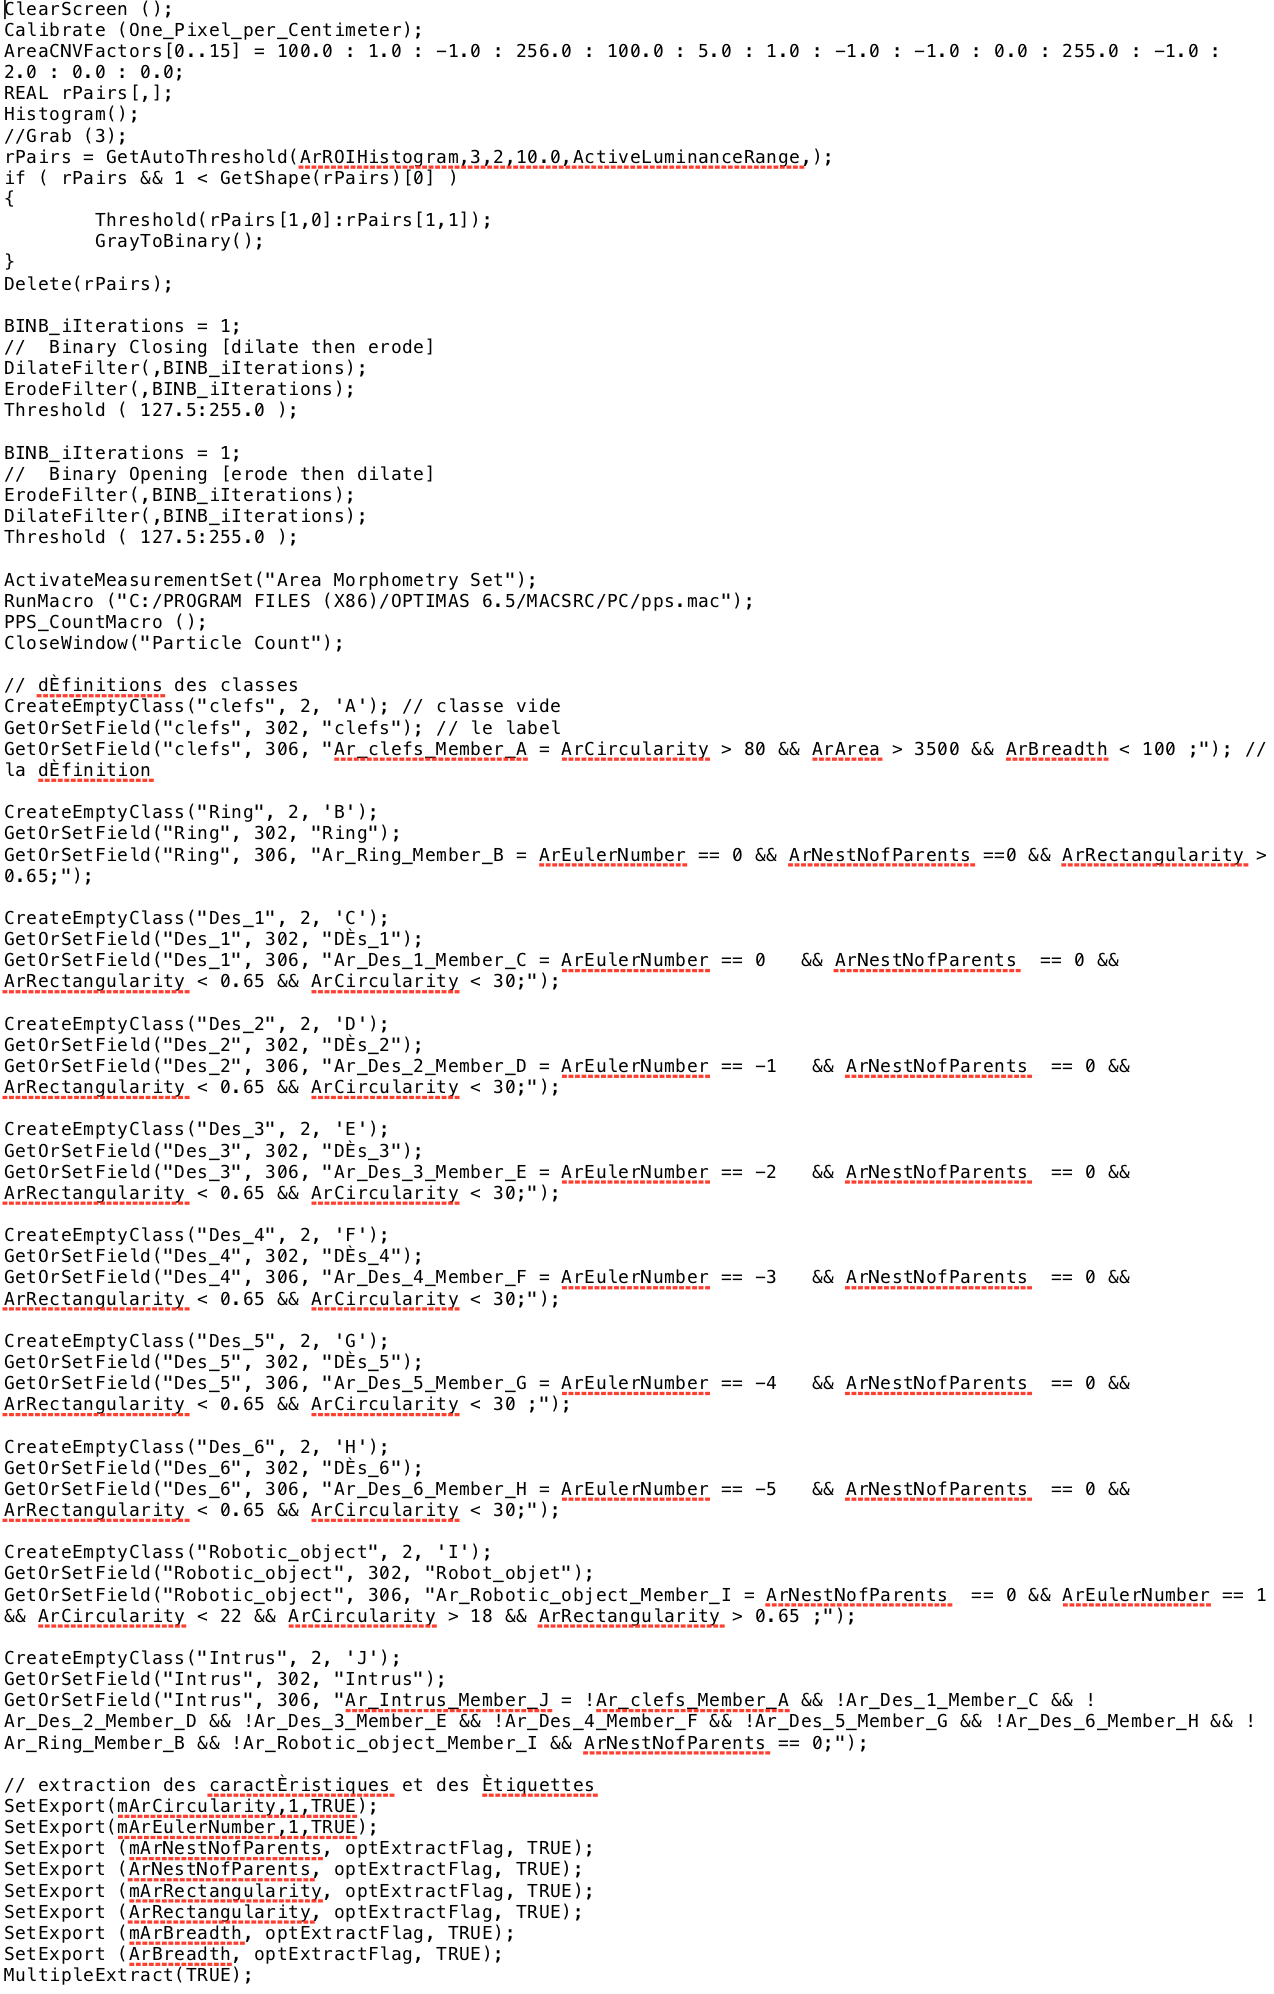
\includegraphics[width=10cm, height=15cm]{images/macro.png}
\caption{Macro de reconnaissance de forme}
\end{figure}

\end{document}

